%-----------------------Homework------------------------------------
%-------------------Arman Shokrollahi---------------------------------

\documentclass[a4 paper]{article}
% Set target color model to RGB
\usepackage{tikz}
\usepackage{amsfonts}
\usepackage{amsthm}
\usepackage{amsmath}
\usepackage{amssymb}
\usepackage{comment}
\usepackage{algorithmic}
\usepackage{verbatim}

\DeclareMathOperator{\st}{\backepsilon^{'}}
\usetikzlibrary{decorations.text,calc,arrows.meta}
\usetikzlibrary{automata,positioning}% Set target color model to RGB
\usepackage{setspace}
%\usepackage[rgb]{xcolor}
%\usepackage{verbatim}
\usepackage{amsgen,amsmath,amstext,amsbsy,amsopn,tikz,amssymb,tkz-linknodes}
\usetikzlibrary{arrows, calc, babel, shapes}
\usepackage{fancyhdr}
\usepackage[colorlinks=true, urlcolor=blue,  linkcolor=blue, citecolor=blue]{hyperref}
\usepackage[colorinlistoftodos]{todonotes}
\usepackage[fulladjust]{marginnote}
\usepackage{rotating}
\usepackage[utf8]{inputenc}
\usepackage[english]{babel}
\usepackage{paracol}
\usepackage{tkz-fct}
\usepackage{fancyhdr}
\usepackage{xstring}
\pagestyle{fancy}
\lhead{\textbf{Viaflow}}
\rhead{\includegraphics[scale=.01]{viaflow.png}}
%\rhead{\textbf{   }}
\usepackage{geometry}
\geometry{
    left = 1.0in,
    right = 1.0in,
    top = 1in,
    head = 1cm,
    foot = .5in,
}
\graphicspath{{images/}}
\hypersetup{%
pdfauthor={Arman Shokrollahi},%
pdftitle={Homework},%
pdfkeywords={Tikz,latex,bootstrap,uncertaintes},%
pdfcreator={PDFLaTeX},%
pdfproducer={PDFLaTeX},%
}
%\usetikzlibrary{shadows}

\usepackage{booktabs}
\newcommand{\ra}[1]{\renewcommand{\arraystretch}{#1}}

      \newtheorem{thm}{Teorema}[section]
      \newtheorem{prop}[thm]{Proposición}
      \newtheorem{lem}[thm]{Lema}
      \newtheorem{cor}[thm]{Corolario}
      \newtheorem{defn}[thm]{Definición}
      \newtheorem{rem}[thm]{Nota}
      \numberwithin{equation}{section}

\newcommand{\homework}[5]{
   \pagestyle{myheadings}
   \thispagestyle{fancy}
   \newpage
   \setcounter{page}{1}
   \noindent
   \begin{center}
   \framebox{
      \vbox{\vspace{4mm}
    \hbox to 1\textwidth { {\bf Paradigma \hfill} }
       \vspace{6mm}
       \hbox to 1\textwidth { {\Large \hfill #1 (#2)  \hfill} }
       \vspace{6mm}
       \hbox to 1\textwidth { {\it Sobrenome: #3 \hfill }
      \vspace{2mm}}
       \hbox to 1\textwidth { {\it Primeiro Nome: #4 \hfill }
      \vspace{2mm}}
       % \hbox to 1\textwidth { {\it ID Number: #5 \hfill }
      %\vspace{2mm}}
 %      \hbox to 1\textwidth { {\it Deadline: #6 \hfill }
 %     \vspace{2mm}}
       %  \hbox to 1\textwidth { {\it Percentage of the final mark: #7 \hfill }
 %     \vspace{2mm}}
      {\bf Respostas}
   }}
   \end{center}
   \markboth{#5 -- #1}{#5 -- #1}
   \vspace*{4mm}
}

\newcommand{\bbF}{\mathbb{F}}
\newcommand{\bbX}{\mathbb{X}}
\newcommand{\bI}{\mathbf{I}}
\newcommand{\bX}{\mathbf{X}}
\newcommand{\bY}{\mathbf{Y}}
\newcommand{\bepsilon}{\boldsymbol{\epsilon}}
\newcommand{\balpha}{\boldsymbol{\alpha}}
\newcommand{\bbeta}{\boldsymbol{\beta}}
\newcommand{\0}{\mathbf{0}}

\newcommand{\problem}[1]{
    {\begin{tikzpicture}[outline/.style={draw=black!75!gray,thick,fill=gray!10!white}]
\node [outline=red] at (0,1) {\bf Questão #1};
\end{tikzpicture}}
}

\newcommand{\solution}[1]{
    {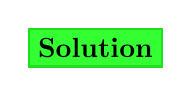
\begin{tikzpicture}[outline/.style={draw=green!75!gray,thick,fill=green!80!white}]
\node [outline=red] at (0,1) {\bf Solution};
\end{tikzpicture}}
}

% Colores
\definecolor{myBlue}{HTML}{027FDF}
\definecolor{negative}{HTML}{181818}
\definecolor{positive}{HTML}{AA3939}

% Recta Real
\newcommand{\reaLine}[2]{
    \node (li) at (#1 - 1.5, 0) {};
    \node (ls) at (#2 + 1.5, 0) {$\mathbb{R}$};
	\draw [>=stealth, <->] (li) -- (ls);
}

%----------------------------------------------------
% Intervalo
% #1 cota inferior
% #2 cota superior
% #3 posición vertical del intervalo
% #4 fill o fill = none o <-, tipo de cota
% #5 fill o fill = none o ->, tipo de cota
% #6 nonInf o inf, tipo de intervalo
\newcommand{\interval}[7]{
    \IfEqCase {#6}{
        {nonInf}{
        \node [circle, draw, #4, line width = 1.5pt, color = #7, inner sep = 0pt, minimum size = 5pt] (ci) at (#1, #3) {};
        \node [circle, draw, #5, line width = 1.5pt, color = #7, inner sep = 0pt, minimum size = 5pt] (cs) at (#2, #3) {};
        \draw [line width = 1.5pt, color = #7] (ci) -- (cs);
        \draw (ci) -- (#1, -.2);
        \node (tag) at (#1, -.4) {#1};
        \draw (cs) -- (#2, -.2);
        \node (tag) at (#2, -.4) {#2};
        }
        {inf}{
        	\IfEqCase {#4}{
            	{<-}{
			        \node [circle, draw, #5, line width = 1.5pt, color = #7, inner sep = 0pt, minimum size = 5pt] (cs) at (#2, #3) {};
                    \draw [>=stealth, #4, line width = 1.5pt, color = #7] (#1 - 1.5, #3) -- (cs);
                    \draw (cs) -- (#2, -.2);
                    \node (tag) at (#2, -.4) {#2};
                }
                {->}{
                	\node [circle, draw, #5, line width = 1.5pt, color = #7, inner sep = 0pt, minimum size = 5pt] (ci) at (#1, #3) {};
                    \draw [>=stealth, ->, line width = 1.5pt, color = #7] (ci) -- (#2 + 1.5, #3);
                    \draw (ci) -- (#1, -.2);
                    \node (tag) at (#1, -.4) {#1};
                }
            }
        }
        }[\PackageError{tree}{Undefined option to intervals: #6}{}]
}
%----------------------------------------------------




\begin{document}
%%%%%%%%%%%%%%%%%%%%%%%%%%%%%%%%%%%%%%%%%%%%%%%%%%%%%%%%
%ADD ACADEMIC YEAR, YOUR DATA
\homework{Prova Pleno}{Novembro/ 2020}{Pinheiro}{Felipe Luís}{Felipe Pinheiro}%{XX$^{\mathbf{th}}$ Month 20XX at 5PM (GMT/BST)}{XX}
%%%%%%%%%%%%%%%%%%%%%%%%%%%%%%%%%%%%%%%%%%%%%%%%%%%%%%%%


%\begin{center}\rule{\textwidth}{0.4pt}\end{center}

%\begin{center}\textbf{\textit{Answer all FIVE questions}
%}\end{center}

\vspace{5mm}
\problem{1}

 Explique o que você entende por MVC (Model-View-Controller), WebAPI (Application Programming Interface) e
ORM (Object Relational Mapper), citando as vantagens de cada um deles.


MVC (Model - View Controller) é um padrão de projeto que divide o projeto em três partes cada uma com atribuiçoes bem especificas de modo a permitir a reutilização de código. As camadas são o modelo, que consiste da parte que possui as regras de negócio, a lógica e as funções do projeto, o controlador, que é a parte que faz o intercambio entre as partes do modelo e visão é a parte do projeto que possui a interface gráfica para a utilização do usuário. 

\vspace{5mm}
\problem{2}

Explique com suas palavras o que você entende pela técnica AJAX, a notação JSON e o protocolo SOAP.

AJAX, acrônimo de Asynchronous JavaScript and XML, consiste em uma tecnica de programação que foi desenvolvida para se criar páginas da web dinâmica, fazendo requisições ao backend sem a necessidade de recarregar toda a página web.

JSON, acrônimo de JavaScript Object Notation, consite em uma notação de objetos, sendo uma forma leve de troca de dados entre aplicações web, sendo de fácil leitura e compreensão para humaos e de fácil interpretação e feração para máquinas.

SOAP, do acrônimo Simple Object Access Protocol, é um protocolo de troca de informação baseada em XML, consistindo em três camadas sendo o envelope, o cabeçalho e o corpo. 

\vspace{5mm}
\problem{3}

 Com base no HTML abaixo, faça um CSS que alinhe os elementos A (menus) e iframe (conteúdo), de modo que o resultado seja o leiaute proposto.

\begin{verbatim}
<!--/* index.html */-->
<html>

<head>
    <title>Minha página</title>
    <link rel='stylesheet' type='text/css' media='screen' href='index.css'>
</head>

<body>
    <nav>
        <a href="#">Frame A</a>
        <a href="#">Frame B</a>
        <a href="#">Frame C</a>
    </nav>

    <iframe id="frmA" src="https://www.paradigmabs.com.br">
    </iframe>

</body>

</html>
\end{verbatim}

\begin{verbatim}
/* Index.css */
body{
    display: grid;
    grid-template-columns: 20% 80% ;
}

nav{
    background-color: lightgray;
}

nav > a{
    margin: 5px;
    padding: 5px;
    display: block;
}

#frmA{
    width: 600px;
}
\end{verbatim}

\vspace{5mm}
\problem{4}

Ainda no exemplo acima, se eu quiser que o elemento A (link) ``Frame A'' abra a página https://ndmais.com.br/ dentro do frame ``frmA'', que marcações no HTML devem ser feitas (sem usar javascript)?

O link Frame A deve ficar com a seguinte estrutura

\begin{verbatim}
<a href="https://ndmais.com.br/" target="frmA">Frame A</a>    
\end{verbatim}



e o Iframe deve ficar com da seguinte forma 

\begin{verbatim}
<iframe id="frmA"name="frmA" src="https://www.paradigmabs.com.br">
</iframe>
\end{verbatim}

\vspace{5mm}
\problem{5}

Com base na marcação abaixo, monte um seletor jQuery que pinte de verde (\#00FF00) todos os elementos LI da segunda DIV (grupo-menu), exceto a que contém o elemento A (Frame E).

\begin{verbatim}
<!--/* index.html */-->
<html>

<head>
    <title>Minha página</title>
</head>

<body>
    <div class="menu">
        <div class="grupo-menu">
            <ul>
                <li><a href="#">Frame A</a></li>
                <li><a href="#">Frame B</a></li>
                <li><a href="#">Frame C</a></li>
            </ul>
        </div>
    </div>
    <div class="menu">
        <div class="grupo-menu">
            <ul>
                <li><a href="#">Frame D</a></li>
                <li><a href="#" name="imprimir">Frame E</a></li>
                <li><a href="#">Frame F</a></li>
            </ul>
        </div>
    </div>
    <div class="menu">
        <div class="grupo-menu">
            <ul>
                <li><a href="#">Frame G</a></li>
                <li><a href="#">Frame H</a></li>
                <li><a href="#">Frame I</a></li>
            </ul>
        </div>
    </div>
</body>

</html>
\end{verbatim}


\vspace{5mm}
\problem{6}

A partir da seguinte cadeia [7, 5, 3, 9, 6, 4, 1], utilize javascript/jquery para percorrer essa lista, localizar e substituir o valor 9 por 55. Localize o valor 4 e remova-o da lista. Imprima a lista final na tela (console.log). O resultado esperado é: [7, 5, 3, 55, 6, 1].

\begin{verbatim}
let numbers = [7, 5, 3, 9, 6, 4, 1];
let i;
for (i = 0; i < numbers.length; i++) {
  if(9 === numbers[i]){
  	numbers[i] = 55;
  }
  if(4 === numbers[i]){
  	numbers.splice(i, 1);
    i--;
  }
}
console.log(numbers);
\end{verbatim}

\vspace{5mm}
\problem{7}

Considere abaixo a tabela de clientes:

\begin{tabular}{|l|l|l|}
\hline
Id & Nome     & IdReferencia \\ \hline
1  & José     & NULL         \\ \hline
2  & Maria    & NULL         \\ \hline
3  & Ana      & 2            \\ \hline
4  & Eduardo  & NULL         \\ \hline
5  & Patrícia & 1            \\ \hline
6  & Alice    & 2            \\ \hline
\end{tabular}

Abaixo você encontra uma consulta que tem por objetivo retornar os clientes que não tem referência (IdReferencia)
com Maria (Id=2):

\begin{verbatim}
SELECT Nome FROM cliente WHERE IdReferencia <> 2;    
\end{verbatim}

Qual será o resultado da consulta? Por quê? Qual seria a melhor maneira de escrever essa consulta?

O resultado dessa consulta será 

\begin{tabular}{|l|}
\hline
Nome     \\ \hline
José     \\ \hline
Maria    \\ \hline
Eduardo  \\ \hline
Patrícia \\ \hline
\end{tabular}

Pois nessa consulta Sql está sendo selecionado todos os elementos que possuem IdReference diferente de 2 e só se está interessado no campo nome da tabela. 

\vspace{5mm}
\problem{8}

Abaixo você encontra uma consulta que tem por objetivo retornar todos os clientes:

\begin{verbatim}
SELECT Id, Nome, IdReferencia FROM cliente;    
\end{verbatim}

Como seria essa consulta se fosse necessário considerar que, se não houver nenhum IdReferencia (NULL), o valor na coluna da consulta deve vir por padrão 0 (zero)?

\begin{verbatim}
SELECT Id, Nome, ISNULL(IdReferencia, 0 )  FROM cliente;
\end{verbatim}

\vspace{5mm}
\problem{9}

Dado um array inteiro sem duplicidade, construa um algoritmo de uma árvore a partir das seguintes regras:

\begin{itemize}
    \item A raiz da árvore deve ser o maior valor da matriz;
    \item Os galhos da esquerda devem ser compostos somente por números à esquerda do valor raiz, na ordem decrescente;
    \item Os galhos da direita devem ser compostos somente por número à direita do valor raiz, na ordem
decrescente;
\end{itemize}

\begin{verbatim}
using System;
using System.Collections.Generic;
using System.Linq;

namespace Paradigma
{
    class Tree
    {
        public Tree(in int node, List<int> right, List<int> left)
        {
            Node = node;
            if (right != null && right.Count != 0)
            {
                var rightNode = right.First();
                right.RemoveAt(0);
                Right = new Tree(rightNode, right, null);
            }
            if (left != null && left.Count != 0)
            {
                var leftNode = left.First();
                left.RemoveAt(0);
                Left = new Tree(leftNode, null, left);
            }
        }

        public int Node { get; }
        public Tree Left { get; set; }
        public Tree Right { get; set; }
    }

    class Program
    {
        static void Main(string[] args)
        {
            Console.WriteLine("Paradigma!");

            var intArray = new[] { 3, 2, 1, 6, 0, 5 };
            var maior = intArray[0];
            var maiorIndex = 0;

            for (var i = 0; i < intArray.Length; i++)
            {
                if (maior < intArray[i])
                {
                    maior = intArray[i];
                    maiorIndex = i;
                }
            }

            Console.WriteLine($"maior: {maior}, Index: {maiorIndex}");

            var right = intArray.Skip(0).Take(maiorIndex).ToList();
            right.Sort();
            right.Reverse();

            var left = intArray.Skip(maiorIndex + 1).Take(intArray.Length - maiorIndex).ToList();
            left.Sort();
            left.Reverse();

            var tree = new Tree(maior, right, left);
        }
    }
}

\end{verbatim}

\vspace{5mm}
\problem{10}

Em C\#, explique a diferença entre os parâmetros de método params, in, ref e out:

Params Usando a palavra-chave params o metodo pode receber um número variavel de argumentos.

Para as palavras-chaves \textit{in}, \textit{ref}, \textit{out} o argumento é passado por referência. Sendo que para o \textit{in}  o argumento não pode ser modificado, para o \textit{ref} o argumento pode ser modificado, enquanto que o \textit{out} o argumento deve ser modificado. 

Tanto o \textit{in} quanto o \textit{ref} a variavel deve ser inicializada antes de ser passada para o metodo, enquanto que para o \textit{out} não é necessário. 

\end{document}